\documentclass[bigger]{beamer}
\usepackage[utf8]{inputenc}
\usepackage{graphicx}
\usepackage{pgfplots}
\usepackage{tabularx}
\usetikzlibrary{calc}


\setbeamertemplate{navigation symbols}{}%remove navigation symbols
\setbeamertemplate{caption}{\raggedright\insertcaption\par}

\begin{document}



\begin{frame}
  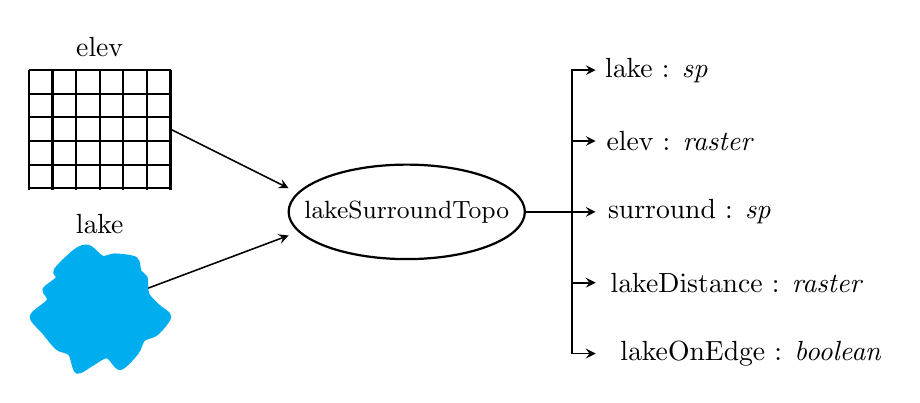
\begin{tikzpicture}[scale = 0.6]
    \draw[>=stealth, ->, line width = 0.2mm] (0, 0) -- (4, 1.5);
    \draw[cyan, ultra thick, domain=0:350, smooth cycle, fill=cyan] 
        plot (\x:1+rnd*0.5);
    \node at (0, 1.75) {lake};
    
    \draw[>=stealth, ->, line width = 0.2mm] (1.5, 3.75) -- (4, 2.5);
    \draw[step=0.5, thick] (-1.5, 2.46) grid (1.5, 5);
    \node at (0, 5.5) {elev};
    
    \draw[thick] (6.5, 2) ellipse (2.5cm and 1cm);
    \node at (6.5, 2) {\small lakeSurroundTopo};
    
    \draw[>=stealth, ->, line width = 0.2mm] (9, 2) -- (10,2)-- (10, 5) -- (10.5, 5);
    \node[align = left] at (11.8, 5) {lake : \emph{sp}};
    
    \draw[>=stealth, ->, line width = 0.2mm] (10, 3.5) -- (10.5, 3.5);
    \node[align = left] at (12.3, 3.5) {elev : \emph{raster}};
    
    \draw[>=stealth, ->, line width = 0.2mm] (10, 2) -- (10.5, 2);
    \node[align = left] at (12.5, 2) {surround : \emph{sp}};
    
    \draw[>=stealth, ->, line width = 0.2mm] (10, 0.5) -- (10.5, 0.5);
    \node[align = left] at (13.5, 0.5) {lakeDistance : \emph{raster}};
    
    \draw[>=stealth, ->, line width = 0.2mm] (10, 2) -- (10,2) -- (10, -1) -- (10.5, -1);
    \node[align = left] at (13.8, -1) {lakeOnEdge : \emph{boolean}};
    
  \end{tikzpicture}

\end{frame}

\begin{frame}
  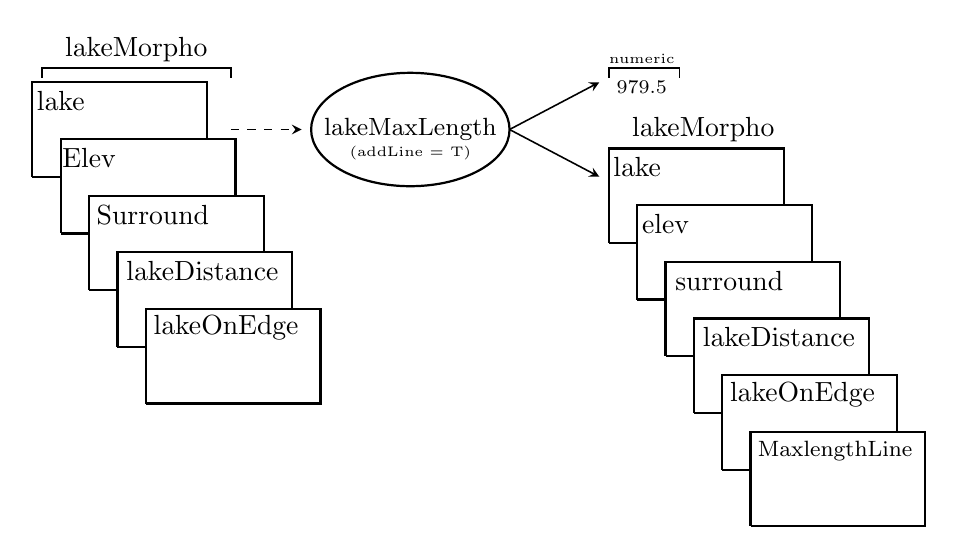
\begin{tikzpicture}[scale = 0.6]
    
    \node at (4.2, 3.7) {lakeMorpho};
    \draw[line width = 0.26mm] (2.2, 3.1) -- (2.2,3.3) -- (6.2,3.3) -- (6.2,3.1);
    \coordinate (boxbot) at (2,1);
    \def\boxwidth{3.7}
    \def\boxheight{2}
    \def\boxsepw{0.6}
    \def\boxseph{-1.2}
    
    \draw[thick] (boxbot) -- 
    ($ (boxbot) + (\boxwidth, 0) $) -- 
    ($ (boxbot) + (\boxwidth, \boxheight) $) -- 
    ($ (boxbot) + (0 , \boxheight) $) -- 
    (boxbot);
    \node at ($ (boxbot) + (0.6, 1.6) $) {lake};
    
    \draw[thick, fill=white] ($ (boxbot) + (\boxsepw, \boxseph) $) -- 
    ($ (boxbot) + (\boxwidth + \boxsepw, 0 + \boxseph) $) -- 
    ($ (boxbot) + (\boxwidth + \boxsepw, \boxheight + \boxseph) $) -- 
    ($ (boxbot) + (0 + \boxsepw , \boxheight + \boxseph) $) -- 
    ($ (boxbot) + (\boxsepw, \boxseph) $);
    \node at ($ (boxbot) + (\boxsepw + 0.6, \boxseph - 0.4 + \boxheight) $) {Elev};
    
    \draw[thick, fill=white] ($ (boxbot) + (2*\boxsepw, 2*\boxseph) $) -- 
    ($ (boxbot) + (\boxwidth + 2*\boxsepw, 0 + 2*\boxseph) $) -- 
    ($ (boxbot) + (\boxwidth + 2*\boxsepw, \boxheight + 2*\boxseph) $) -- 
    ($ (boxbot) + (0 + 2*\boxsepw , \boxheight + 2*\boxseph) $) -- 
    ($ (boxbot) + (2*\boxsepw, 2*\boxseph) $);
    \node at ($ (boxbot) + (2*\boxsepw + 1.35, 2*\boxseph - 0.4 + \boxheight) $) {Surround};
    
    \draw[thick, fill=white] ($ (boxbot) + (3*\boxsepw, 3*\boxseph) $) -- 
    ($ (boxbot) + (\boxwidth + 3*\boxsepw, 0 + 3*\boxseph) $) -- 
    ($ (boxbot) + (\boxwidth + 3*\boxsepw, \boxheight + 3*\boxseph) $) -- 
    ($ (boxbot) + (0 + 3*\boxsepw , \boxheight + 3*\boxseph) $) -- 
    ($ (boxbot) + (3*\boxsepw, 3*\boxseph) $);
    \node at ($ (boxbot) + (3*\boxsepw + 1.8, 3*\boxseph - 0.4 + \boxheight) $) {lakeDistance};
    
    \draw[thick, fill=white] ($ (boxbot) + (4*\boxsepw, 4*\boxseph) $) -- 
    ($ (boxbot) + (\boxwidth + 4*\boxsepw, 0 + 4*\boxseph) $) -- 
    ($ (boxbot) + (\boxwidth + 4*\boxsepw, \boxheight + 4*\boxseph) $) -- 
    ($ (boxbot) + (0 + 4*\boxsepw , \boxheight + 4*\boxseph) $) -- 
    ($ (boxbot) + (4*\boxsepw, 4*\boxseph) $);
    \node at ($ (boxbot) + (4*\boxsepw + 1.7, 4*\boxseph - 0.4 + \boxheight) $) {lakeOnEdge};
    
    
    \draw[>=stealth, ->, line width = 0.2mm, dashed] (6.2, 2) -- (7.7, 2);
    \draw[thick] (10, 2) ellipse (2.1cm and 1.2cm);
    \node[align=left] at (10, 2) {\small lakeMaxLength};
    \node[align=left] at (10, 1.5) {\tiny (addLine = T)};
    
    \draw[>=stealth, ->, line width = 0.2mm] (12.1, 2) -- (14, 3);
    \node[align=left] at (14.9, 3.5) {\tiny numeric};
    \draw[line width = 0.2mm] (14.2, 3.1) -- (14.2,3.3) -- (15.7,3.3) -- (15.7,3.1);
    \node[align=left] at (14.9, 2.9) {\scriptsize 979.5};
    
    \node at (16.2, 2) {lakeMorpho};
    \draw[>=stealth, ->, line width = 0.2mm] (12.1, 2) -- (14, 1);
    \coordinate (boxbot) at (14 + 0.2, 1 - 0.7 * \boxheight);
    \def\boxwidth{3.7}
    \def\boxheight{2}
    \def\boxsepw{0.6}
    \def\boxseph{-1.2}
    
    \draw[thick] (boxbot) -- 
    ($ (boxbot) + (\boxwidth, 0) $) -- 
    ($ (boxbot) + (\boxwidth, \boxheight) $) -- 
    ($ (boxbot) + (0 , \boxheight) $) -- 
    (boxbot);
    \node at ($ (boxbot) + (0.6, 1.6) $) {lake};
    
    \draw[thick, fill=white] ($ (boxbot) + (\boxsepw, \boxseph) $) -- 
    ($ (boxbot) + (\boxwidth + \boxsepw, 0 + \boxseph) $) -- 
    ($ (boxbot) + (\boxwidth + \boxsepw, \boxheight + \boxseph) $) -- 
    ($ (boxbot) + (0 + \boxsepw , \boxheight + \boxseph) $) -- 
    ($ (boxbot) + (\boxsepw, \boxseph) $);
    \node at ($ (boxbot) + (\boxsepw + 0.6, \boxseph - 0.4 + \boxheight) $) {elev};
    
    \draw[thick, fill=white] ($ (boxbot) + (2*\boxsepw, 2*\boxseph) $) -- 
    ($ (boxbot) + (\boxwidth + 2*\boxsepw, 0 + 2*\boxseph) $) -- 
    ($ (boxbot) + (\boxwidth + 2*\boxsepw, \boxheight + 2*\boxseph) $) -- 
    ($ (boxbot) + (0 + 2*\boxsepw , \boxheight + 2*\boxseph) $) -- 
    ($ (boxbot) + (2*\boxsepw, 2*\boxseph) $);
    \node at ($ (boxbot) + (2*\boxsepw + 1.35, 2*\boxseph - 0.4 + \boxheight) $) {surround};
    
    \draw[thick, fill=white] ($ (boxbot) + (3*\boxsepw, 3*\boxseph) $) -- 
    ($ (boxbot) + (\boxwidth + 3*\boxsepw, 0 + 3*\boxseph) $) -- 
    ($ (boxbot) + (\boxwidth + 3*\boxsepw, \boxheight + 3*\boxseph) $) -- 
    ($ (boxbot) + (0 + 3*\boxsepw , \boxheight + 3*\boxseph) $) -- 
    ($ (boxbot) + (3*\boxsepw, 3*\boxseph) $);
    \node at ($ (boxbot) + (3*\boxsepw + 1.8, 3*\boxseph - 0.4 + \boxheight) $) {lakeDistance};
    
    \draw[thick, fill=white] ($ (boxbot) + (4*\boxsepw, 4*\boxseph) $) -- 
    ($ (boxbot) + (\boxwidth + 4*\boxsepw, 0 + 4*\boxseph) $) -- 
    ($ (boxbot) + (\boxwidth + 4*\boxsepw, \boxheight + 4*\boxseph) $) -- 
    ($ (boxbot) + (0 + 4*\boxsepw , \boxheight + 4*\boxseph) $) -- 
    ($ (boxbot) + (4*\boxsepw, 4*\boxseph) $);
    \node at ($ (boxbot) + (4*\boxsepw + 1.7, 4*\boxseph - 0.4 + \boxheight) $) {lakeOnEdge};
    
    \draw[thick, fill=white] ($ (boxbot) + (5*\boxsepw, 5*\boxseph) $) -- 
    ($ (boxbot) + (\boxwidth + 5*\boxsepw, 0 + 5*\boxseph) $) -- 
    ($ (boxbot) + (\boxwidth + 5*\boxsepw, \boxheight + 5*\boxseph) $) -- 
    ($ (boxbot) + (0 + 5*\boxsepw , \boxheight + 5*\boxseph) $) -- 
    ($ (boxbot) + (5*\boxsepw, 5*\boxseph) $);
    \node at ($ (boxbot) + (5*\boxsepw + 1.79, 5*\boxseph - 0.4 + \boxheight) $) {\footnotesize MaxlengthLine};
    
  \end{tikzpicture}

\end{frame}



% \begin{frame}
%   \begin{tikzpicture}[scale = 0.6]
%     \draw[>=stealth, ->, line width = 0.2mm] (0, 0) -- (4, 1.5);
%     \draw[cyan, ultra thick, domain=0:350, smooth cycle, fill=cyan] 
%         plot (\x:1+rnd*0.5);
%     \node at (0, 1.75) {lake};
%     
%     \draw[>=stealth, ->, line width = 0.2mm] (1.5, 3.75) -- (4, 2.5);
%     \draw[step=0.5, thick] (-1.5, 2.46) grid (1.5, 5);
%     \node at (0, 5.5) {elev};
%     
%     \draw[thick] (4,1) -- (6,1) -- (6,3) -- (4,3) -- (4,1);
%     \draw[thick] (4.2,0.8) -- (6.2,0.8) -- (6.2,2.8) -- (4.2,2.8) -- (4.2,0.8);
%     \node at (5, 3.5) {lakeMorpho};
%     
%     \draw[>=stealth, ->, line width = 0.2mm, dashed] (6.2, 2) -- (8, 2);
%     \draw[thick] (10, 2) ellipse (2cm and 1cm);
%     \node at (10, 2) {\small lakeMaxWidth};
%     
%     \draw[>=stealth, ->, line width = 0.2mm] (12, 2) -- (13,2)-- (13, 4) -- (14, 4);
%     \node[align = left] at (12.8, 5) {addLine \\  TRUE};
%     
%     \draw[>=stealth, ->, line width = 0.2mm] (12, 2) -- (13,2) -- (13, 0) -- (14, 0);
%     \node[align = left] at (12.8, -1) {addLine \\  FALSE};
%     
%     \draw[thick] (14,3) -- (16,3) -- (16,5) -- (14,5) -- (14,3);
%     \draw[thick] (14.2,2.8) -- (16.2,2.8) -- (16.2,4.8) -- (14.2,4.8) -- (14.2,2.8);
%     \draw[thick] (14.4,2.6) -- (16.4,2.6) -- (16.4,4.6) -- (14.4,4.6) -- (14.4,2.6);
%     
%     \draw[thick] (14,-1) -- (16,-1) -- (16,1) -- (14,1) -- (14,-1);
%     \draw[thick] (14.2,-1.2) -- (16.2,-1.2) -- (16.2,0.8) -- (14.2,0.8) -- (14.2,-1.2);
%     
%   \end{tikzpicture}
% 
% \end{frame}

\end{document}
